%************************************************
\chapter{Evaluation}
\label{chapter:evaluation}
%************************************************

The primary contribution of this thesis is a recursive implementation
of a reflective planning layer that controls a deliberative planning
process.  Because of the recursive nature of this implementation, a
super-reflective layer is also used to control and learn about the
reflective planning process.  The benefit of adding each additional
reflective layer is that more can be learned from each deliberative
failure by adding each additional reflective layer, but there is a
computational trade-off in that each additional reflective layer also
increases the computational complexity of the overall architecture.
This chapter evaluates the Emotion Machine cognitive architecture
contribution of this thesis by measuring the computational complexity
introduced by adding additional reflective planning layers to the SALS
deliberative planning process.  First, the perceptual inputs to each
planning layer are described and evaluated.  Next, the time-complexity
of natural language plan interpretation at each reflective layer is
evaluated.  Finally, the performance of the SALS virtual machine at
efficiently executing parallel processes concurrently on multicore and
hyperthreaded CPUs is evaluated.

\section{Complexity of Perceptual Inputs}

The key to beginning to think about the computational complexity in a
given planning layer of the SALS cognitive architecture is in
considering the perceptual inputs to that layer.  The perceptual
inputs to a planning layer determine the complexity of the goals that
the planner can attempt to accomplish or avoid as well as the
complexity of the causal models that the planning layer will construct
for a given rule-learning algorithm.  There are two different types of
inputs to a SALS planning layer from the layer below:
\begin{packed_enumerate}
\item{Procedurally Reflective Event Streams}
\item{Direct Read Access}
\end{packed_enumerate}
The first, procedurally reflective event streams, is the basis of the
asynchronous learning from experience that was discussed in detail in
{\mbox{\autoref{chapter:learning_asynchronously_from_experience}}}.
To briefly review, learning from experience asynchronously abstracts a
small subset of all possible partial states from a stream of events
that represent changes that have occurred in the knowledge base that
the planning layer is trying to control.  These abstracted partial
state events are woven together with resource activation and
completion events through a rule-learning algorithm to learn abstract
hypothetical models of resource executions in the layer below.  These
hypothetical models are used by the planning layer to imagine the
effects of plans before they are executed.  The second type of input
to a planning layer, direct read access, allows an executing plan to
access the real-time state of the knowledge base that it is trying to
control.  The important thing to realize about both of these different
methods of accessing and referring to the knowledge base in the layer
below is that both of these methods work exclusively through a small
subset of possible partial state abstractions.
{\mbox{\autoref{chapter:learning_from_being_told}}} describes two
specific types of these partial state abstractions that can be
perceived by the planning layer: (1) the ``{\tt{relationship}}''
expression, and (2) the ``{\tt{property}}'' expression.  The fact that
all perceptual input to a planning layer is limited to these specific
types of partial state abstractions limits the complexity of the
control problem that the planning layer confronts.  For example,
because of the simplicity of the included partial states, the SALS AI
cannot directly pursue a single goal to create a stack of three
blocks.  Instead, the deliberative layer of the SALS AI must be
instructed, by either a user or the reflective layer, to pursue two
goals composed of these simpler partial states to make a plan to stack
three blocks: (1) ``{\tt{Block-1 to be on Block-2}}'' and (2)
``{\tt{Block-2 to be on Block-3}}.''  The important point is not that
the abstracted partial states are currently simple but instead that
the planning layer is \emph{limited} to perceiving its problem domain
through partial state abstractions that reduce the complexity of the
problem domain to a set of symbolic reifications that either exist or
do not exist in the control domain.

Knowledge in a SALS planning layer includes plans, goals, a planner,
and other knowledge used in the planning process.  In addition to the
planning objects, knowledge in a planning layer includes symbolically
reified references to the knowledge in the layer below.  Keeping clear
distinctions between knowledge in different layers is critical to
reducing the potential complexity of the SALS architecture.  For
example, while the deliberative plan knowledge base references
physical knowledge in the learned reactive physical knowledge base,
the deliberative plan knowledge does not actually contain physical
knowledge.  Instead, the deliberative plan knowledge base contains
symbolized reifications of potential partial states of the physical
knowledge base.
{\mbox{\autoref{figure:deliberative_physical_partial_state_reification}}}
shows a simple example of a deliberative goal that refers to a
potential partial state of the physical knowledge base and how this
partial state is symbolically reified in the deliberative layer.
\begin{figure}
\centering
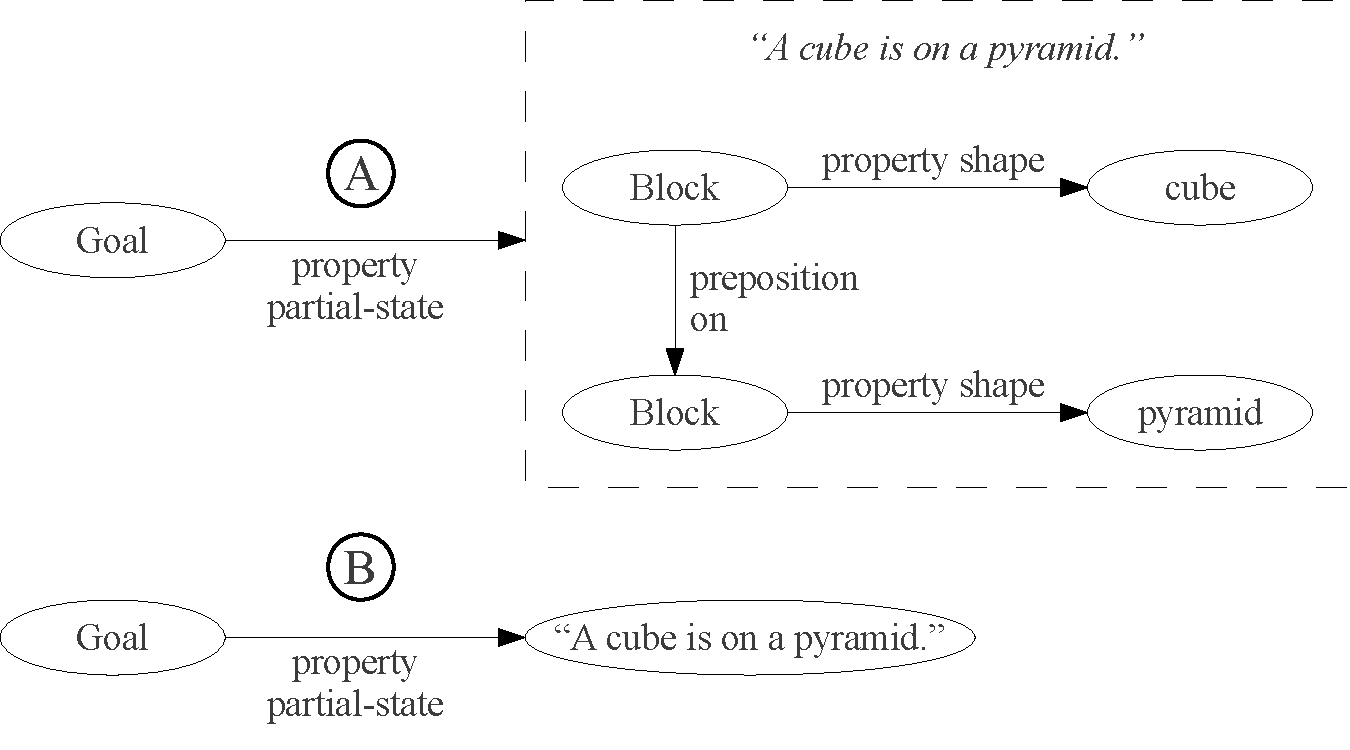
\includegraphics[width=10cm]{gfx/deliberative_physical_partial_state_reification}
\caption[Deliberative physical partial state
  reification.]{Deliberative physical partial state reification.  (A)
  A visualization of the idea that a deliberative goal object can
  refer to a potential partial state of the physical knowledge base.
  (B) The actual representation of a deliberative goal object that has
  a symbolic ``{\tt{partial-state}}'' property, the symbolic phrase,
  ``{\tt{a cube is on a pyramid}},'' being a reference to the
  potential physical partial state visualized in (A).  Each planning
  layer is limited to reflecting upon reified symbols that refer to
  partial states in the layer below and not the complexity of the
  partial states themselves.}
\label{figure:deliberative_physical_partial_state_reification}
\end{figure}
Because deliberative knowledge only contains symbols that refer to
physical partial states, this allows the deliberative layer to ignore
the internal details of the physical partial state and simply treat
the goal symbolically.

The number of partial states that are abstracted from any given
knowledge base depends primarily on the structure of the knowledge
within that knowledge base and whether or not that structure contains
the types of partial states that the SALS AI is prepared to abstract.
The partial states that are currently included in the SALS AI are
meant to be both specific enough to handle the simple types of
meaningful relationships that have been engineered to exist in each
knowledge base while being general enough to leave room for those
serendipitous abstractions that have not been engineered but may still
end up being useful to the rule-learning algorithm in building causal
models of resource executions.
{\mbox{\autoref{table:frames_slots_partial_states}}} shows how the
sizes of the knowledge bases in the layers of the SALS AI relate to
the numbers of partial states that are abstracted from these knowledge
bases by the layers above.
\begin{table}
\centering
\begin{tabular}{|l|c|c|}
\hline
\emph{Knowledge Base}     & \emph{Frames} & \emph{Partial States Abstracted} \\
\hline
Learned Reactive Physical & 6             & 174                              \\
\hline
Deliberative Plan         & 120           & 122                              \\
\hline
Reflective Plan           & 224           & 103                              \\
\hline
Super-Reflective Plan     & 208           & {\scriptsize{\emph{N/A}}}        \\
\hline
\end{tabular}
\caption[A comparison of the sizes of knowledge bases in the layers of
  the SALS AI to the numbers of partial states that are abstracted
  from these knowledge bases.]{A comparison of the sizes of knowledge
  bases in the layers of the SALS AI to the numbers of partial states
  that are abstracted from these knowledge bases.  Notice that the
  number of partial states abstracted from any given knowledge base is
  not directly a function of the number of frames in the knowledge
  base.  For example, the learned reactive physical knowledge base
  contains very few frames with a highly interconnected structure that
  contains many of the types of partial states that SALS is designed
  to abstract, while the plan knowledge bases contain a relatively
  large number of frames with fewer and more sparse relationships that
  result in fewer abstracted partial states.  The super-reflective
  layer is currently the highest layer in the SALS AI, so no partial
  states are currently abstracted from the super-reflective plan
  knowledge base.}
\label{table:frames_slots_partial_states}
\end{table}
Notice that the total number of partial states that are abstracted
from any given knowledge base is not directly a function of the number
of frames in that knowledge base.  For example, the learned reactive
physical knowledge base contains relatively few frames with a highly
interconnected structure that contains many of the types of partial
states that SALS is designed to abstract, while the plan knowledge
bases contain a relatively large number of frames with fewer and more
sparse relationships that result in fewer abstracted partial states.
The number of partial states that are the perceptual input to each
planning layer \emph{decreases} as subsequent layers of reflective
planning are added to the SALS AI.  In general, this rule may not hold
for two reasons:
\begin{packed_enumerate}
\item{Planning layers may become more interconnected as the AI gains
  experience.}
\item{More types of partial states may be added to the SALS AI in the
  future.}
\end{packed_enumerate}
Both of these situations may cause the total number of partial states
abstracted from a plan knowledge base to grow intractably.  Because of
this potential problem, an eye must be kept on these numbers when
designing new types of knowledge representations for each planning
layer in the SALS AI.  A general solution would consider the number of
perceptual inputs to a planning layer as a control problem in itself.
Currently, the number of perceptual inputs to a planning layer in the
SALS architecture grows sub-linearly with each subsequently higher
layer of reflective control.

\section{Complexity of Plan Interpretation}

While the perceptual inputs to higher-level planning layers in the
SALS AI are currently kept at a tractable sub-linear complexity for
each additional layer, there is still the question of how the planning
process scales in time-complexity for each subsequently higher layer
in the SALS AI.  The planning process can be broken down into two main
stages:
\begin{packed_enumerate}
\item{Plan Interpretation and Imagination}
\item{Plan Execution}
\end{packed_enumerate}
Plan interpretation and imagination involves a search through a number
of possible partial interpretations of natural language phrases
expressed in the simple SALS template matching programming language,
which has been described in
{\mbox{\autoref{chapter:learning_from_being_told}}}.
To briefly review, the search through possible natural language
interpretations involves finding analogies to other already known
natural language plans that match the phrase that is currently being
interpreted.  The interpretation process (1) considers the current
state of the domain that the planning layer is trying to control, (2)
ignores interpretations that compile to programs that are imagined to
have bugs, such as passing the wrong argument type to a low-level
function, and also (3) ignores interpretations that do not accomplish
the current goals of the planning layer or fail to avoid negative
goals.  Depending on the type of reflectively chosen planning process,
plan execution generally occurs after a natural language plan has been
interpreted, all natural language ambiguity has been compiled away,
and the plan has been deemed relevant to either accomplishing positive
goals or avoiding negative goals.

Because the plan interpretation process requires a search through a
number of ambiguously specified analogies to previously known natural
language plans, this process can potentially have a considerable
time-complexity as natural language phrases become longer and more
complex at higher level reflective layers.  There is a distinction
between the time-complexity of learning from being told and learning
from experience.  When a planning layer in the SALS AI learns from
experience, a stream of procedurally reflective trace events are
received from changes in the layer below and these are abstracted into
partial states that are symbolically reified before being stored in
the causal hypotheses of the planning layer.  When these hypotheses
are used to hypothesize the effects of a plan, only the reified symbol
that refers to the partial state in the layer below is stored as
related to the plan in the planning layer.  When a reflective layer
above the planning layer learns from experience, it receives a stream
of events that includes the new relationship between the plan and the
symbolized partial state in the planning layer.  The reflective layer
itself symbolically reifies this partial state of the planning layer.
As this process continues up through each additional reflective
planning layer, each reflective layer performs one symbolic
reification that is again symbolically reified by the next layer as
part of a higher-level partial state that ultimately may refer,
through symbolic reference, to the original physical knowledge, the
ground knowledge layer.\footnote{It should be clear that reflective
  knowledge has no requirement to be ultimately grounded in physical
  knowledge.  Knowledge can ultimately refer to the partial states of
  any layer.  See \cite{minsky:2011} for a more detailed discussion of
  interior grounding in reflective and self-reflective thinking.}
{\mbox{\autoref{figure:multiple_layers_of_symbolic_reification}}}
shows an example of three layers of recursive symbolic reification.
\begin{figure}
\centering
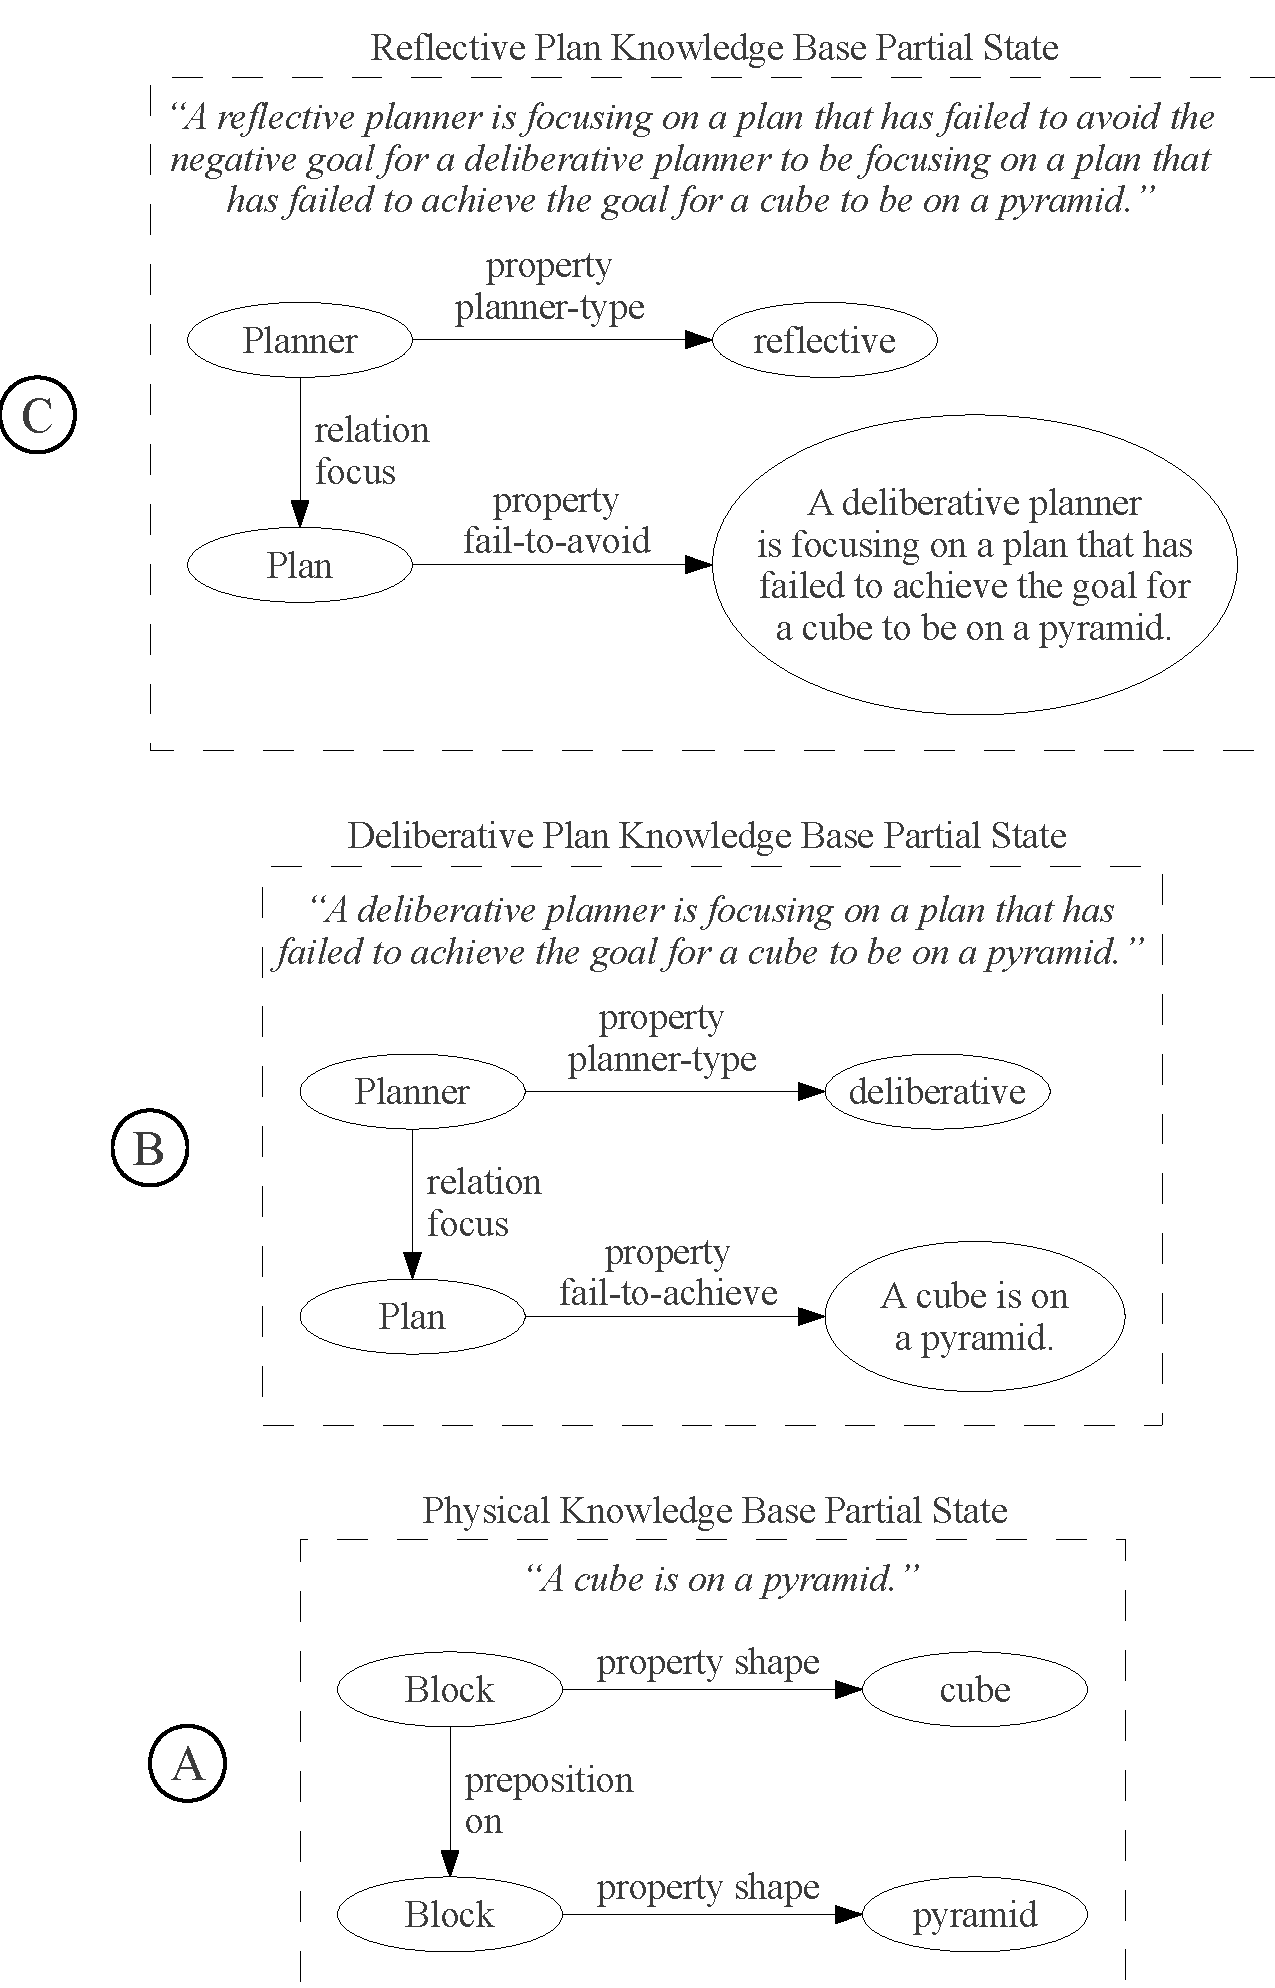
\includegraphics[width=10cm]{gfx/multiple_layers_of_symbolic_reification}
\caption[Three layers of knowledge that form a hierarchy of reified
  symbolic reference.]{Three layers of knowledge that form a hierarchy
  of reified symbolic reference.  (A) A physical partial state that is
  symbolically reified in the deliberative layer.  (B) A deliberative
  partial state that is symbolically reified in the reflective layer.
  The deliberative partial state contains the symbolic reification of
  \emph{A}.  (C) A reflective partial state that is symbolically
  reified in the super-reflective layer.  The reflective partial state
  contains the symbolic reification of \emph{B}.  Also, the reflective
  partial state indirectly references \emph{A} through its direct
  reference to \emph{B}.}
\label{figure:multiple_layers_of_symbolic_reification}
\end{figure}
The following are three pieces of knowledge from different layers of
the SALS AI, where the first piece of knowledge is symbolically
referred to by the second, and the second is symbolically referred to
by the third:
\begin{packed_enumerate}
\item{Physical Knowledge: ``{\tt{a pyramid is on a cube}}.''}
\item{Deliberative Knowledge: ``{\tt{a deliberative planner is
      focusing on a plan that has failed to achieve the goal for a
      cube to be on a pyramid}}.''}
\item{Reflective Knowledge: ``{\tt{a reflective planner is focusing on
      a plan that has failed to avoid the negative goal for a
      deliberative planner to be focusing on a plan that has failed to
      achieve the goal for a cube to be on a pyramid}}.''}
\end{packed_enumerate}
To continue to reference physical knowledge in higher layers, the
natural language phrases become longer, more complex, and take more
time to interpret and compile to their reified symbolic forms.
{\mbox{\autoref{table:time_complexity_of_recursive_reification}}}
shows a comparison of the time-complexities for interpreting each of
these three natural language phrases.
\begin{table}
\centering
\begin{tabular}{|r l|l|r|}
\hline
           &\emph{Referent} &\emph{Reference}  &\emph{Execution Nodes} \\
\hline
\emph{(A)} &Physical        & Deliberative     & 18                    \\
\hline
\emph{(B)} &Deliberative    & Reflective       & 92                    \\
\hline
\emph{(C)} &Reflective      & Super-Reflective & 125                   \\
\hline
\end{tabular}
\caption[A comparison of the execution node time-complexity of three
  different natural language phrases that reference one another in
  recursive hierarchy.]{A comparison of the execution node
  time-complexity of three different natural language phrases that
  reference one another in recursive hierarchy.  (A) A natural
  language phrase that compiles to a physical knowledge partial state
  in the deliberative layer.  (B) A natural language phrase that
  compiles to a deliberative knowledge partial state in the reflective
  layer that includes a symbolically reified reference to the physical
  partial state in \emph{A}.  (C) A natural language phrase that
  compiles to a reflective knowledge partial state in the
  super-reflective layer that includes a symbolically reified direct
  reference to the deliberative partial state in \emph{B} and an
  indirect reference to the physical partial state in \emph{A}.}
\label{table:time_complexity_of_recursive_reification}
\end{table}
As can be seen in this table, interpreting, imagining and compiling
natural language phrases that refer to physical knowledge at higher
layers of reflective planning grows quickly in time-complexity in just
the first few layers.  For this reason, while the SALS AI is capable
of interpreting these types of natural language phrases that reference
knowledge in multiple layers below a given planning layer, these types
of natural language phrases are strictly avoided in the implementation
of the natural language planning algorithms in the reflective and
super-reflective layers.  These types of hierarchical references
through all of the layers below any given planning layer are commonly
abstracted by the process of learning by experience, where the time
complexity is sub-linear per additional layer, but while these
knowledge references are possible to express in natural language to
the SALS AI, they are avoided in the definitions of the plans that
define the planning processes because of this problematic scaling
factor in learning these types of complex knowledge from being told.

The only knowledge references that are told to the planning layers in
the SALS AI are the goals in the immediate layer below the planning
layer that the planning layer should try to accomplish or avoid.
Examples of these goals are as follows:
\begin{packed_enumerate}
\item{Reflective Plan: ``{\tt{want a cube to be on a pyramid}}.''}
\item{Reflective Plan: ``{\tt{want a pyramid to be on a cube}}.''}
\item{Super-Reflective Plan: ``{\tt{Avoid a deliberative planner being
      focused on a plan that has failed}}.''}
\end{packed_enumerate}
{\mbox{\autoref{table:time_complexity_of_interpreting_goals}}} shows
the time-complexities of interpreting these natural language phrases
in the reflective and super-reflective layers that specify goals for
the deliberative and reflective layers, respectively.
\begin{table}
\centering
\begin{tabular}{|r l|r|}
\hline
           &\emph{Plan Layer}     &\emph{Execution Nodes} \\
\hline
\emph{(A)} &Reflective Plan       & 18                    \\
\hline
\emph{(B)} &Reflective Plan       & 18                    \\
\hline
\emph{(C)} &Super-Reflective Plan & 18                    \\
\hline
\end{tabular}
\caption[Time-complexities of interpreting natural language plans that
  specify goals in only the immediate layer below the
  plan.]{Time-complexities of interpreting natural language plans that
  specify goals in only the immediate layer below the plan.  Note that
  the time-complexity of interpreting these natural language phrases
  that specify goals in the deliberative and reflective layers have
  equal time-complexity.  This result implies a linear increase in
  time-complexity for each additional layer of plans that specify
  goals in only the one layer immediately below the plans.  As
  previously shown, plans that specify goals that indirectly reference
  knowledge in layers multiple levels below the plan have a greater
  than linear increase in time-complexity.}
\label{table:time_complexity_of_interpreting_goals}
\end{table}
The time-complexity of interpreting these natural language phrases
that specify goals in the deliberative and reflective layers have
equal time-complexity.  This result implies a linear time-complexity
for specifying more goals in each additional reflective layer in the
SALS AI.

Because the natural language plans in the reflective and
super-reflective layers that define the planning algorithms are
independent of any specific goals that they may be trying to
accomplish, these plans do not contain any knowledge references at
all.  Instead, the natural language plans that define the planning
algorithms are simply composed of resource activations in the
immediate layer below.  The following are plans of action in each of
the three planning layers of the SALS AI:
\begin{packed_enumerate}
\item{Deliberative: ``{\tt{stack a cube on a pyramid}}.''}
\item{Reflective: ``{\tt{find recent plan to accomplish my positive
      goals}}.''}
\item{Super-Reflective: ``{\tt{find recent plan to avoid my negative
      goals}}.''}
\end{packed_enumerate}
{\mbox{\autoref{table:time_complexity_of_plans_for_action_in_each_layer}}}
shows the time-complexity of interpreting these plans for action in
the each of the three planning layers of the SALS AI.
\begin{table}
\centering
\begin{tabular}{|r l|r|}
\hline
           &\emph{Plan Layer}              &\emph{Execution Nodes} \\
\hline
\emph{(A)} &Deliberative Physical Plan     & 3003                  \\
\hline
\emph{(B)} &Reflective Planning Plan       & 170                   \\
\hline
\emph{(C)} &Super-Reflective Planning Plan & 152                   \\
\hline
\end{tabular}
\caption[The time-complexity of interpreting plans for action in the
  three planning layers in the SALS AI.]{The time-complexity of
  interpreting plans for action in the three planning layers of the
  SALS AI.  (A) The deliberative physical plans take much more
  time-complexity to interpret because they are idiosyncratic to the
  Blocks World planning domain, including specific references to
  shapes, colors, and prepositional relationships.  Each different
  problem domain will have a different set of deliberative plans in
  order to manipulate that domain.  (B) The reflective planning plans
  are interpreted and become the deliberative planning processes.  (C)
  The super-reflective planning plans are interpreted and become the
  reflective planning processes.  Notice that the reflective planning
  plan is roughly of the same time-complexity as the super-reflective
  planning plan.  The fact that planning plans are of the same
  time-complexity independent of their interpretation layer implies a
  linear increase in overall complexity as more planning layers are
  added to the SALS AI.}
\label{table:time_complexity_of_plans_for_action_in_each_layer}
\end{table}
The reflective planning plans are roughly of the same time-complexity
as the super-reflective planning plans.  The fact that planning plans
are of the same time-complexity independent of their interpretation
layer implies a linear increase in overall complexity as more planning
layers are added to the SALS AI.

\section{Efficiency of Concurrent Execution}

\begin{filecontents}{parallel_processing_speedup_amd64_8_core_pthread.data}
1 1.00
2 2.00
3 3.00
4 4.00
5 4.99
6 5.97
7 6.94
8 7.90
9 6.81
10 7.15
11 7.35
12 7.47
13 7.44
14 7.61
15 7.69
16 7.75
17 7.56
18 7.71
19 7.80
20 7.85
21 7.79
22 7.84
23 7.89
24 7.94
25 7.82
26 7.86
27 7.87
28 7.89
29 7.90
30 7.93
31 7.95
32 7.95
33 7.86
34 7.91
35 7.94
36 7.94
37 7.95
38 7.94
39 7.96
40 7.93
41 7.92
42 7.94
43 7.96
44 7.96
45 7.97
46 7.97
47 7.97
48 7.96
49 7.94
50 7.96
51 7.97
52 7.97
53 7.97
54 7.97
55 7.97
56 7.97
57 7.97
58 7.97
59 7.97
60 7.98
61 7.97
62 7.98
63 7.98
64 7.98
\end{filecontents}

\begin{filecontents}{parallel_processing_speedup_amd64_8_core.data}
1 1.00
2 1.91
3 2.37
4 2.16
5 2.54
6 2.96
7 3.85
8 3.94
9 3.78
10 3.57
11 3.68
12 3.82
13 3.85
14 3.88
15 3.93
16 4.13
17 3.99
18 4.40
19 4.28
20 4.18
21 4.12
22 4.15
23 4.01
24 4.03
25 4.28
26 4.41
27 3.59
28 3.66
29 3.73
30 3.76
31 3.93
32 3.86
33 3.91
\end{filecontents}

\begin{filecontents}{parallel_processing_speedup_amd64_8_core_no_gc.data}
1 1.00
2 1.99
3 2.47
4 2.24
5 2.65
6 3.12
7 4.14
8 4.22
9 4.07
10 3.84
11 3.93
12 4.10
13 4.13
14 4.25
15 4.28
16 4.54
17 4.42
18 4.60
19 4.63
20 4.56
21 4.42
22 4.45
23 4.47
24 4.45
25 4.73
26 4.96
27 3.93
28 3.97
29 4.06
30 4.09
31 4.21
32 4.19
33 4.20
\end{filecontents}

\begin{filecontents}{parallel_processing_speedup_intel_4_core_pthread.data}
1 1.00
2 1.80
3 2.52
4 3.22
5 2.85
6 3.29
7 3.31
8 3.37
9 3.29
10 3.35
11 3.35
12 3.39
13 3.40
14 3.42
15 3.42
16 3.43
17 3.41
18 3.43
19 3.43
20 3.44
21 3.44
22 3.46
23 3.45
24 3.46
25 3.44
26 3.45
27 3.45
28 3.44
29 3.45
30 3.46
31 3.46
32 3.45
33 3.44
34 3.45
35 3.45
36 3.45
37 3.45
38 3.45
39 3.45
40 3.46
41 3.46
42 3.46
43 3.46
44 3.46
45 3.46
46 3.47
47 3.47
48 3.46
49 3.47
50 3.46
51 3.46
52 3.46
53 3.46
54 3.46
55 3.46
56 3.46
57 3.46
58 3.46
59 3.46
60 3.46
61 3.47
62 3.46
63 3.46
64 3.45
\end{filecontents}

\begin{filecontents}{parallel_processing_speedup_intel_4_core.data}
1 1.00
2 1.42
3 1.90
4 2.34
5 2.66
6 3.07
7 3.14
8 3.26
9 3.23
10 3.03
11 3.18
12 3.60
13 3.34
14 3.34
15 3.09
16 3.31
17 3.17
18 3.13
19 3.17
20 3.16
21 3.29
22 3.26
23 3.26
24 3.23
25 3.59
26 3.51
27 3.48
28 3.47
29 3.06
30 3.17
31 2.98
32 3.29
33 3.23
34 3.61
35 3.63
36 3.40
37 3.11
38 3.06
39 3.10
40 3.17
41 3.29
42 2.98
43 3.19
44 3.11
45 3.06
46 3.22
\end{filecontents}

\begin{filecontents}{parallel_processing_speedup_intel_4_core_no_gc.data}
1 1.00
2 1.43
3 1.93
4 2.39
5 2.71
6 3.15
7 3.26
8 3.36
9 3.35
10 3.10
11 3.31
12 3.69
13 3.48
14 3.47
15 3.22
16 3.39
17 3.27
18 3.25
19 3.29
20 3.25
21 3.36
22 3.35
23 3.37
24 3.36
25 3.80
26 3.66
27 3.68
28 3.60
29 3.21
30 3.31
31 3.10
32 3.44
33 3.34
34 3.83
35 3.80
36 3.55
37 3.31
38 3.20
39 3.22
40 3.30
41 3.42
42 3.09
43 3.29
44 3.22
45 3.17
46 3.33
\end{filecontents}

The SALS virtual machine is built to take advantage of multiple
processors and multicore processors with hardware hyperthreads.
{\mbox{\autoref{chapter:virtual_machine_and_programming_language}}}
discusses the details of the parallel and concurrent processing
features of the SALS virtual machine and low-level Lisp-like
programming language.  To briefly review, to reduce cache misses, a
separate memory pool is allocated for each separate hardware
hyperthread in the target hardware platform.  Each of these memory
pools is allocated a virtual processor object in the SALS virtual
machine.  Each concurrent virtual processor has a separate scheduler
that simulates parallelism for a number of parallel processes, called
{\emph{fibers}} to distinguish them from the low-level operating
system thread objects.  The SALS garbage collector is a concurrent
implementation of a tricolor garbage collection algorithm.
{\mbox{\autoref{figure:parallel_processing_speedup}}} compares the
speedup gained by executing multiple processes in parallel on the SALS
virtual machine to the optimal speedup that could be expected.  These
tests were executed on a GNU/Linux system.
\begin{figure}
\centering
\begin{tikzpicture}
\begin{axis}[%
scale only axis,
width=1.0\textwidth,
height=0.4\textheight,
xmin=0, xmax=64,
ymin=0, ymax=4,
xlabel={Process Count},
ylabel={Speedup Factor},
legend entries={Optimal GNU/Linux,SALS Virtual Machine,SALS Virtual Machine (No GC)},
legend style={nodes=right},
legend pos= south east,
grid = major,
grid style={dashed, gray!30},
/pgfplots/xtick={0,8,...,64}]
        
%\addplot [color=black, solid]
\addplot[dashed] plot[color=black, mark=*, mark size=1] file {parallel_processing_speedup_intel_4_core_pthread.data};

%\addplot [color=black, solid]
\addplot plot[color=black, mark=*, mark size=1] file {parallel_processing_speedup_intel_4_core.data};

%\addplot [color=black, solid]
\addplot[dotted] plot[color=black, mark=*, mark size=1] file {parallel_processing_speedup_intel_4_core_no_gc.data};

\end{axis}
\end{tikzpicture}
\caption[The speedup gained by executing multiple processes
  concurrently in the SALS virtual machine.]{The speedup gained by
  executing multiple processes concurrently in the SALS virtual
  machine.  The solid line plot represents the speedup experienced by
  the SALS AI as more fiber processes are executed in parallel.  The
  dashed line plot represents the optimal speedup that can be expected
  on this specific hardware.  Each parallel process in this experiment
  is performing the same numerical processing task on memory that is
  independent of other tasks.  The number of computations performed by
  a single parallel process is used as the unity standard for the
  speedup comparisons.  These tests were run on an Intel Core i7
  processor with 4 cores, each with 2 hardware hyperthreads.  In these
  tests, 8 virtual processors and 8 memory pools were allocated, one
  for each hyperthread in the target hardware platform.  Each test was
  performed 100 times to average out variations caused by intermittent
  garbage collections.  The optimal speedup is calculated by a short C
  program that uses POSIX thread primitives, optimized C arithmetic,
  and no memory allocation or garbage collection.  The SALS AI has a
  small overhead for each additional parallel process, which is seen
  by the downward slope of the solid plot.  The SALS virtual machine
  performs most efficiently on this hardware with 7 parallel fibers
  executing.  These tests were executed on a GNU/Linux system.}
\label{figure:parallel_processing_speedup}
\end{figure}
\begin{figure}
\centering
\begin{tikzpicture}
\begin{axis}[%
scale only axis,
width=1.0\textwidth,
height=0.4\textheight,
xmin=0, xmax=64,
ymin=0, ymax=10,
xlabel={Process Count},
ylabel={Speedup Factor},
legend entries={Optimal GNU/Linux,SALS Virtual Machine,SALS Virtual Machine (No GC)},
legend style={nodes=right},
legend pos= south east,
grid = major,
grid style={dashed, gray!30},
/pgfplots/xtick={0,8,...,64}]
        
%\addplot [color=black, solid]
\addplot[dashed] plot[color=black, mark=*, mark size=1] file {parallel_processing_speedup_amd64_8_core_pthread.data};

%\addplot [color=black, solid]
\addplot plot[color=black, mark=*, mark size=1] file {parallel_processing_speedup_amd64_8_core.data};

%\addplot [color=black, solid]
\addplot[dotted] plot[color=black, mark=*, mark size=1] file {parallel_processing_speedup_amd64_8_core_no_gc.data};

\end{axis}
\end{tikzpicture}
\caption{Parallel processing speedup on Dual AMD64 CPUs with 4 cores
  each.}
\label{figure:parallel_processing_speedup_amd64_8_core}
\end{figure}
Each parallel process in this experiment is performing the same
numerical processing task on memory that is independent of other
tasks.  The number of computations performed by a single parallel
process is used as the unity standard for the speedup comparisons.
These tests were run on an Intel Core i7 processor with 4 cores, each
with 2 hardware hyperthreads.  In these tests, 8 virtual processors
and 8 memory pools were allocated, one for each hyperthread in the
target hardware platform.  Each test was performed 100 times to
average out variations caused by intermittent garbage collections.
The optimal speedup is calculated by a short C program that uses POSIX
thread primitives, optimized C arithmetic, and no memory allocation or
garbage collection.  The SALS AI has a small overhead for each
additional parallel process, which is seen by the downward slope of
the solid plot.

All of the time-complexities that have been presented in this chapter
do not incorporate any speedup that is gained by using concurrent or
parallel hardware.  There are many aspects of the SALS AI that take
advantage of the concurrent processing capabilities of the SALS
virtual machine.  For example, because the SALS natural language
planning language is a simple functional grammar, any ambiguous
interpretations are performed in parallel processes in the SALS
virtual machine.  Also, each planning layer contains two asynchronous
learning stages that each contain two parallel agencies that
concurrently process streams of procedurally reflective trace events.


%% \begin{table}
%% \centering
%% \begin{tabular}{|l|r|r|}
%% \hline
%%                  &Execution Nodes &Plan Analogies \\
%% \hline
%% Super Reflective & 152            & 11            \\
%% \hline
%% Reflective       & 170            & 13            \\
%% \hline
%% Deliberative     & 3003           & 240           \\
%% \hline
%% \end{tabular}

%% \begin{tabular}{|l|r|r|}
%% \hline
%%                  &Version Spaces &Hypotheses \\
%% \hline
%% Super Reflective &               &           \\
%% \hline
%% Reflective       &               &           \\
%% \hline
%% Deliberative     &               &           \\
%% \hline
%% \end{tabular}
%% \caption{The number of execution nodes and plan analogies that were
%%   made during in different stages of plan processing in the different
%%   planning layers during a planning scenario involving the super
%%   reflective layer interpreting and compiling a plan to ``find and
%%   execute a recently learned plan that avoids a negative reflective
%%   goal.''  The execution of the super reflective plan becomes the
%%   reflective planning process.  The reflective planning process
%%   searches through deliberative plans until it finds a plan to ``find
%%   and execute a recently learned plan for accomplishing a positive
%%   deliberative goal.''  The execution of the reflective plan becomes
%%   the deliberative planning process.  The deliberative planning
%%   process interprets and imagines a plan to ``stack a cube on a
%%   pyramid,'' which is hypothesized to accomplish a positive
%%   deliberative goal.}
%% \label{table:plan_interpretation_computational_complexity_of_layers}
%% \end{table}

%% The knowledge at higher layers of reflective control is symbolically
%% reified by being filtered through the perceptions of lower level
%% layers.

%% {\mbox{\autoref{figure:meta_meta_knowledge}}} shows a visualization of
%% an example of reflective knowledge that references potential
%% deliberative knowledge, while this potential deliberative knowledge
%% references potential physical knowledge.
%% \begin{figure}
%% \centering
%% 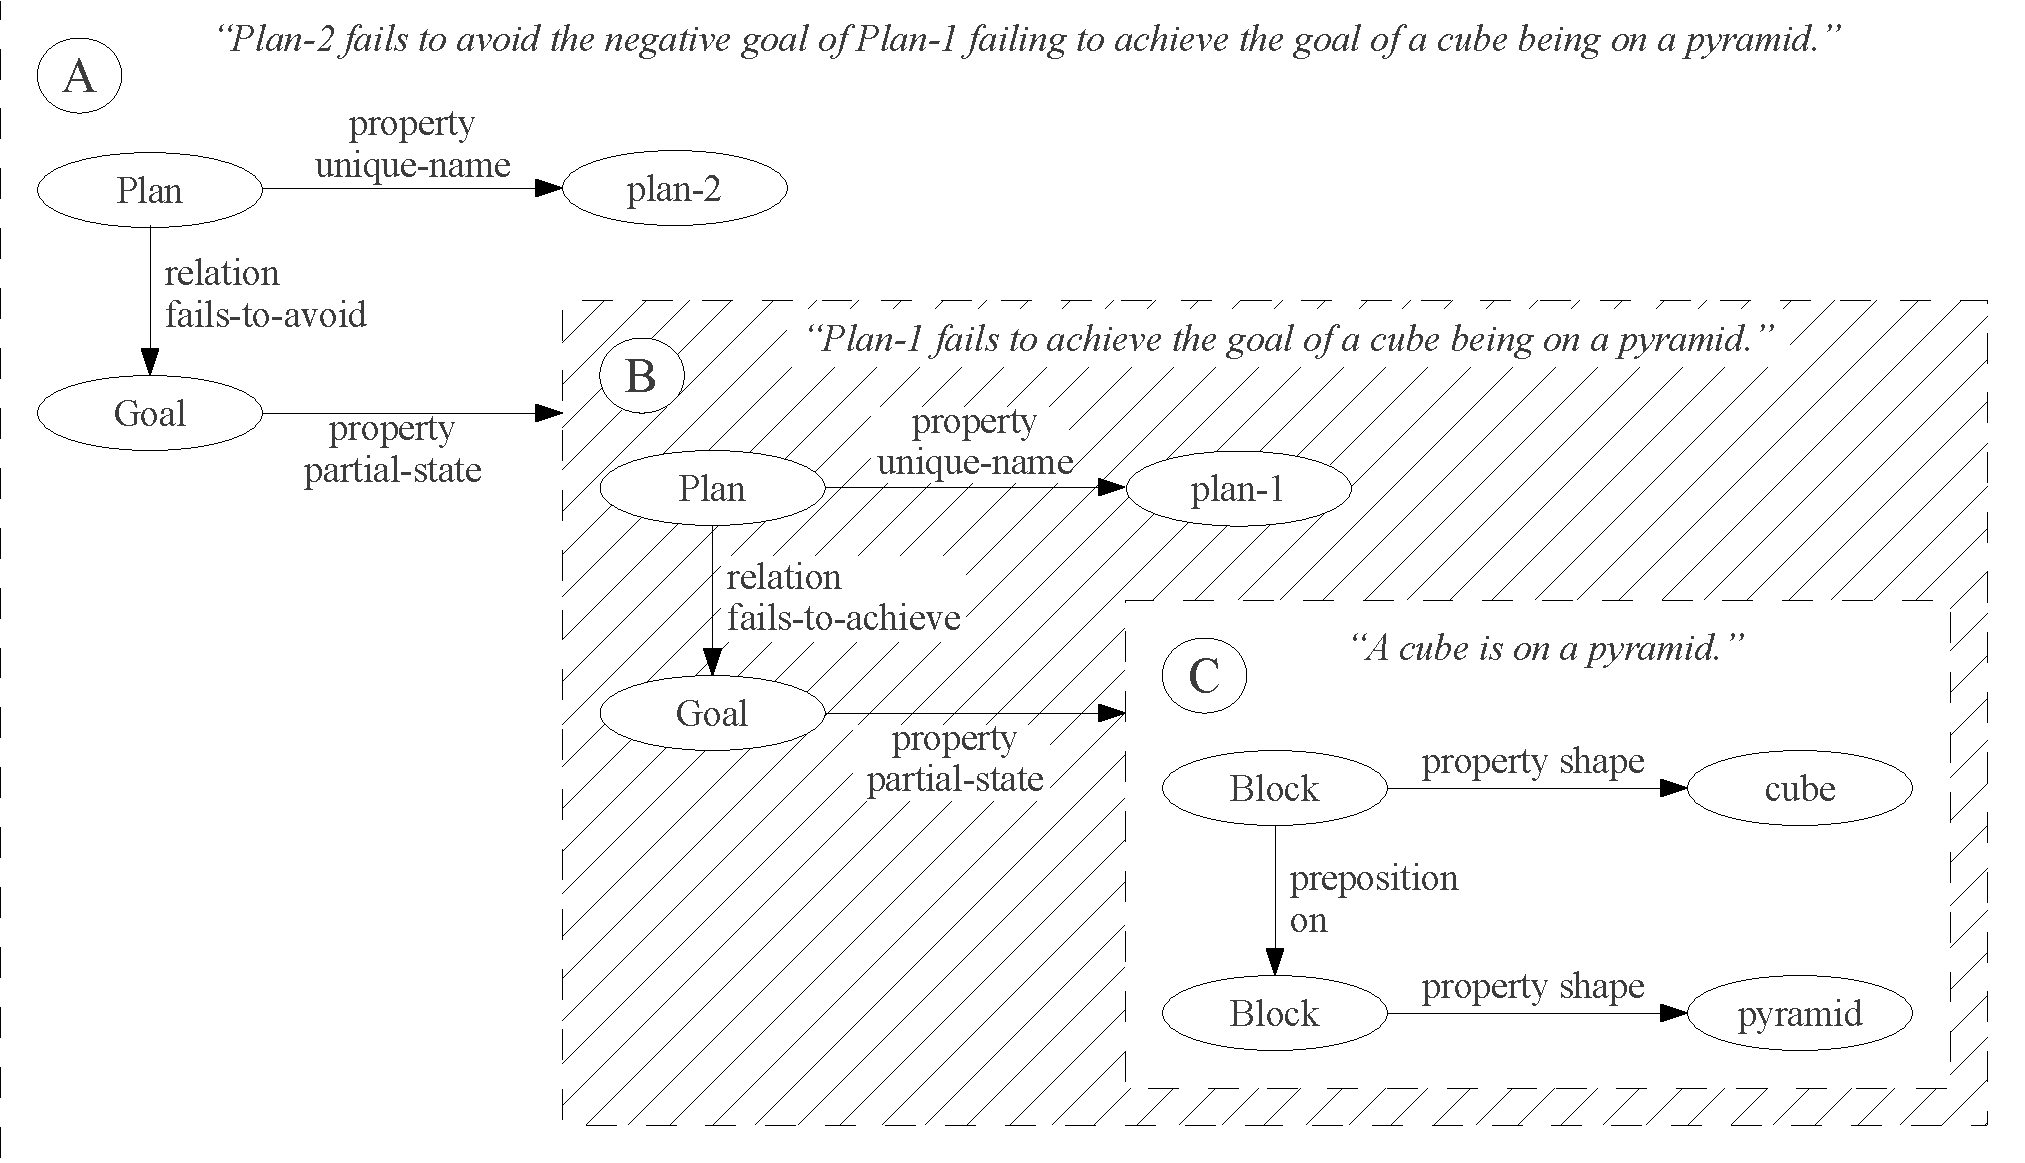
\includegraphics[width=12cm]{gfx/meta_meta_knowledge}
%% \caption[A visualization of the idea that a reflective partial state
%%   can indirectly reference physical knowledge.]{A visualization of the
%%   idea that a reflective partial state can indirectly reference
%%   physical knowledge.}
%% \label{figure:meta_meta_knowledge}
%% \end{figure}



%% \begin{samepage}
%% \begin{Verbatim}
%% [exists 
%%   [relationship planner property planner_type reflective
%%                 relation focus_plan
%%                 plan property failed_to_avoid 
%%     [relationship planner property planner_type deliberative
%%                   relation focus_plan
%%                   plan property failed_to_achieve
%%       [relationship block property shape cube
%%                     preposition on
%%                     block property shape pyramid]]]]
%% \end{Verbatim}
%% \end{samepage}


%% has the potential to be more complex and thus more difficult to reason
%% about than the knowledge in the layers below that knowledge.  For
%% example, a partial state of the physical problem domain can be a
%% simple relationship such as ``a pyramid being on a cube.''  Since the
%% deliberative layer contains meta-physical knowledge, or ``knowledge
%% about physical knowledge,'' a simple deliberative partial state could
%% be that ``a deliberative plan fails to accomplish the goal for a cube
%% to be on a pyramid.''  This deliberative knowledge appears at first
%% glance to be more complex than the physical knowledge that it is about
%% because it contains, in some sense, the physical knowledge as well as
%% additional relationships between this physical knowledge and a plan
%% and a goal.  Further, the reflective layer contains meta-meta-physical
%% knowledge, so a piece of reflective knowledge could be that ``a
%% reflective plan fails to avoid the negative goal of a deliberative
%% plan failing to achieve the goal of a cube being on a pyramid.''
%% {\mbox{\autoref{figure:meta_meta_knowledge}}} shows a visualization of
%% this example of meta-meta-knowledge with a reflective partial state
%% that references a deliberative partial state that references a
%% physical partial state.
%% \begin{figure}
%% \centering
%% 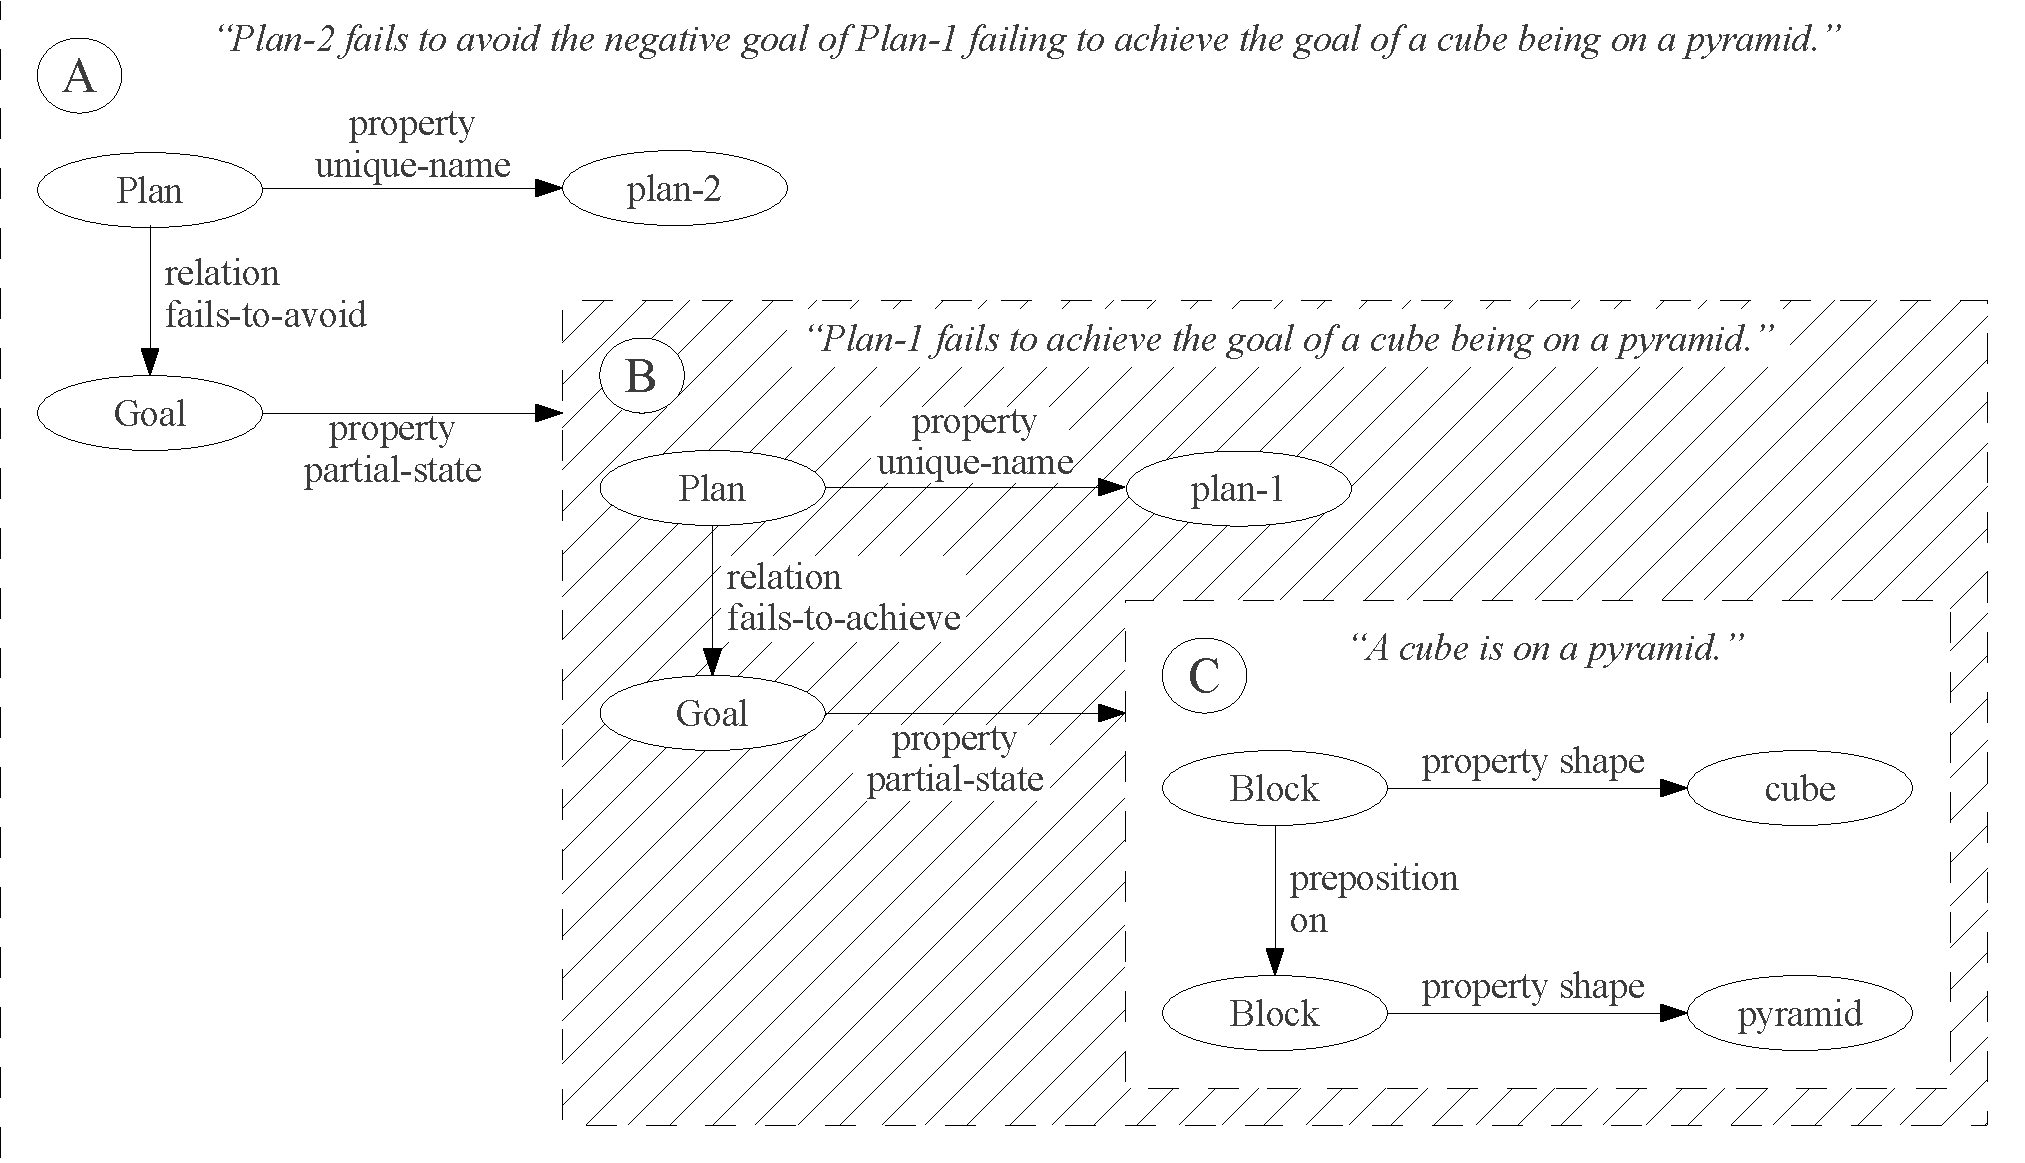
\includegraphics[width=12cm]{gfx/meta_meta_knowledge}
%% \caption{Meta-meta-knowledge of (A) a reflective partial state that
%%   references (B) a deliberative partial state that references (C) a
%%   physical partial state.}
%% \label{figure:meta_meta_knowledge}
%% \end{figure}
%% {\mbox{\autoref{table:meta_meta_knowledge_complexity}}} shows the
%% computational complexity of evaluating each one of these increasingly
%% complex forms of knowledge.  The phrase, ``a cube is on a pyramid,''
%% is interpreted in the deliberative layer and results in the following
%% SALS program:

%% \begin{samepage}
%% \begin{Verbatim}
%% [exists
%%   [relationship block property shape 'cube'
%%                 preposition on
%%                 block property shape 'pyramid']]
%% \end{Verbatim}
%% \end{samepage}

%% \noindent The phrase, ``a deliberative planner is focusing on a plan
%% that is hypothesized to cause a cube to be on a pyramid,'' is
%% interpreted by the reflective layer and refers to a partial state of
%% the deliberative plan knowledge base, which results in the following
%% SALS program:

%% \begin{samepage}
%% \begin{Verbatim}
%% [exists
%%   [relationship planner property planner_type deliberative
%%                 relation focus_plan
%%                 plan property hypothesized_to_cause
%%                 [relationship block property shape 'cube'
%%                               preposition on
%%                               block property shape 'pyramid']]]
%% \end{Verbatim}
%% \end{samepage}

%% \noindent The phrase, ``a reflective planner is focusing on a plan
%% that is hypothesized to cause a deliberative planner to be focusing on
%% a plan that is hypothesized to cause a cube to be on a pyramid,'' is
%% interpreted by the super-reflective layer and refers to a partial
%% state of the reflective plan knowledge base, which results in the
%% following SALS program:

%% \begin{samepage}
%% \begin{Verbatim}
%% [exists 
%%   [relationship planner property planner_type reflective
%%                 relation focus_plan
%%                 plan property hypothesized_to_cause
%%     [relationship planner property planner_type deliberative
%%                   relation focus_plan
%%                   plan property hypothesized_to_cause
%%       [relationship block property shape 'cube'
%%                     preposition on
%%                     block property shape 'pyramid']]]]
%% \end{Verbatim}
%% \end{samepage}



%% \begin{table}
%% \centering
%% \begin{tabular}{|l|c|c|}
%% \hline
%%                  &Execution Nodes   &Plan Analogies    \\
%%                  &{\scriptsize{(Imagine/Execute)}} &{\scriptsize{(Imagine/Execute)}} \\
%% \hline
%% Deliberative     & 18/12            & 2/0              \\
%% \hline
%% Reflective       & 98/22            & 10/0             \\
%% \hline
%% Super Reflective & 348/32           & 27/0             \\
%% \hline
%% \end{tabular}
%% \caption{The number of execution nodes and plan analogies that were
%%   made interpreting a deliberative statement about physical knowledge,
%%   a reflective meta-knowledge statement about deliberative knowledge
%%   that references the same physical knowledge, and a super-reflective
%%   meta-meta-knowledge statement that references the same physical
%%   knowledge through deliberative knowledge.}
%% \label{table:meta_meta_knowledge_complexity}
%% \end{table}




%% \begin{table}
%% \centering
%% \begin{tabular}{|l|r|r|}
%% \hline
%%                  &Execution Nodes &Plan Analogies \\
%% \hline
%% Super Reflective & 152            & 11            \\
%% \hline
%% Reflective       & 170            & 13            \\
%% \hline
%% Deliberative     & 3003           & 240           \\
%% \hline
%% \end{tabular}

%% \begin{tabular}{|l|r|r|}
%% \hline
%%                  &Version Spaces &Hypotheses \\
%% \hline
%% Super Reflective &               &           \\
%% \hline
%% Reflective       &               &           \\
%% \hline
%% Deliberative     &               &           \\
%% \hline
%% \end{tabular}
%% \caption{The number of execution nodes and plan analogies that were
%%   made during in different stages of plan processing in the different
%%   planning layers during a planning scenario involving the super
%%   reflective layer interpreting and compiling a plan to ``find and
%%   execute a recently learned plan that avoids a negative reflective
%%   goal.''  The execution of the super reflective plan becomes the
%%   reflective planning process.  The reflective planning process
%%   searches through deliberative plans until it finds a plan to ``find
%%   and execute a recently learned plan for accomplishing a positive
%%   deliberative goal.''  The execution of the reflective plan becomes
%%   the deliberative planning process.  The deliberative planning
%%   process interprets and imagines a plan to ``stack a cube on a
%%   pyramid,'' which is hypothesized to accomplish a positive
%%   deliberative goal.}
%% \label{table:plan_interpretation_computational_complexity_of_layers}
%% \end{table}

%% \section{Old Stuff}

%% This dissertation consists of four contributions that work together to
%% form the SALS AI.  From the low-level virtual machine and Lisp-like
%% programming language to the reflective and super-reflective layers of
%% the Emotion Machine cognitive architecture, it is difficult to
%% evaluate all aspects of the SALS AI by a single simple metric.
%% Therefore, this chapter presents a number of different metrics that
%% are used to evaluate the four contributions:
%% \begin{packed_enumerate}
%% \item{\emph{Emotion Machine Cognitive Architecture}: The primary
%%   contribution of this thesis is a recursive implementation of a
%%   reflective planning layer that controls a deliberative planning
%%   process.  Because of the recursive nature of the implementation, a
%%   super-reflective layer is also used to control and learn about the
%%   reflective planning process.  The benefit of adding each additional
%%   reflective layer is that more can be learned from each deliberative
%%   failure by adding each additional reflective layer, but there is a
%%   computational trade-off in that each additional reflective layer
%%   also increases the computational complexity of the overall
%%   architecture.  This chapter evaluates the Emotion Machine cognitive
%%   architectural component of the SALS AI by asking the following
%%   question: What is the increase in computational complexity
%%   introduced by adding additional reflective planning layers to the
%%   basic deliberative planning process?}
%% \item{\emph{Learning from Being Told Natural Language Plans}: The
%%   ability of each planning layer in the SALS AI to interpret and
%%   imagine the effects of ambiguous natural language plans relies on a
%%   search through possible interpretations of each natural language
%%   phrase in any given plan.  This search would quickly become
%%   intractable if it were not controlled by a number of different types
%%   of low-level programmatic constraints.  Only those natural language
%%   plan interpretations that make programmatic sense according to these
%%   constraints are further considered for imagination or execution.  In
%%   practice, each low-level constraint helps to reduce the overall
%%   search complexity by varying amounts depending on the domain of
%%   control, whether the natural language plan is describing a control
%%   process for the physical, deliberative, or reflective knowledge
%%   domains.  This chapter shows empirical results that compare the size
%%   of the overall natural language plan interpretation search with and
%%   without each of these constraints for the control of each knowledge
%%   domain in the SALS AI.  This chapter also discusses the trade-offs
%%   between introducing language specific constraints, such as
%%   English-only semantics or syntax, versus purely programmatic
%%   constraints that keep the SALS natural planning language as it is
%%   currently applicable to all natural human languages.}
%% \item{\emph{Learning Asynchronously from Experience}: The ability of
%%   each planning layer in the SALS AI to asynchronously abstract the
%%   partial state events in its control knowledge domain as well as
%%   asynchronously learn rule-based causal models of resource
%%   activations of the layer below introduces two potentially
%%   problematic scaling factors for the computational complexity of the
%%   overall SALS AI.  Firstly, the number of partial states in arbitrary
%%   knowledge domains could in the worst case introduce a factorial
%%   growth with the size of the knowledge domain and the size of the
%%   partial states being abstracted.  As factorial growth would be an
%%   intractable scaling factor for the computational complexity, this
%%   chapter shows empirical evidence for the actual scaling factors for
%%   abstracting partial states from each of the control knowledge
%%   domains, including the physical, deliberative, and reflective
%%   knowledge domains.  The causal hypothesis rule-learning algorithm
%%   could potentially even have a worse scaling factor that is a
%%   multiplier on the number of partial states abstracted in the first
%%   asynchronous stage in the SALS AI's learning from experience.  This
%%   chapter will also present empirical evidence of the actual scaling
%%   factor introduced by the conjunctive rule-learning algorithm
%%   employed in learning causal models of resource activations in the
%%   SALS AI for each planning layer, including the deliberative,
%%   reflective, and super-reflective layers.}
%% \item{\emph{Virtual Machine and Programming Language}: The SALS AI is
%%   constructed on a low-level virtual machine and Lisp-like programming
%%   language that takes advantage of multithreaded and multicore CPUs.
%%   The SALS virtual machine executes concurrent bytecode processes that
%%   are called ``fibers,'' which are an abstraction of the POSIX threads
%%   provided by the underlying operating system.  In order to minimize
%%   hyperthread-specific cache-miss effects for each concurrently
%%   executing fiber, a separate memory pool is allocated for each
%%   hardware hyperthread in each CPU core in the underlying hardware
%%   platform.  The SALS virtual machine performs dynamic load balancing
%%   in order to take advantage of as many CPU cores as possible while
%%   executing multiple fibers.  Also, the SALS virtual machine includes
%%   a concurrent tricolor garbage collection algorithm that has been
%%   optimized to be used over multiple memory pools.  In a perfect
%%   symmetric multiprocessing (SMP) system, executing $N$ fibers on $N$
%%   processors should have a constant time-complexity, but modern
%%   multithreaded and multicore CPUs have shared caches between
%%   hyperthreads and cores, which makes systems based on these CPUs less
%%   than ideal SMPs.  Furthermore, mutual exclusion (mutex) locks
%%   required for garbage collection slow down garbage collection across
%%   multiple memory pools by a factor depending on the number of
%%   cross-references between pools.  This chapter empirically evaluates
%%   how the SALS virtual machine performs at minimizing these cache-miss
%%   and locking effects on an Intel Core i7 CPU, which has 4 cores, each
%%   with 2 hyperthreads, while executing various numbers of concurrent
%%   fibers.}
%% \end{packed_enumerate}

%% \section{Computational Complexity of Reflective Layers}

%% What is the increase in computational complexity introduced by adding
%% additional reflective planning layers to the basic deliberative
%% planning process?  The answer to this question is not at first obvious
%% because of the exponentially larger state-space confronted by each
%% higher planning layer.  The result is that each additional layer adds
%% a roughly linear increase in computational complexity to the overall
%% architecture.  This chapter discusses how the increased computational
%% complexity of each additional reflective planning layer is kept from
%% becoming exponential in the SALS AI.  This chapter also discusses how
%% using concurrent hardware in order to separately simulate each
%% additional reflective layer has the potential to reduce the overall
%% time-complexity of the architecture to sub-linear per additional
%% layer.

%% The SALS AI consists of 100 parallel heterogeneous resources,
%% organized into 29 agencies, which comprise the 5 layers.  The causal
%% procedurally reflective tracing features of the SALS virtual machine
%% that have been described in
%% {\mbox{\autoref{chapter:virtual_machine_and_programming_language}}}
%% allow for the run-time evaluation of each separate causally scoped
%% component of the SALS AI.  In the evaluation of the complexity of each
%% additional reflective layer, the following execution events are
%% measured:
%% \begin{packed_enumerate}
%% \item{Memory Allocation in Bytes}
%% \item{Garbage Collection in Bytes}
%% \item{Bytecode Execution Count}
%% \item{Semantic Frame Slot Mutations}
%% \item{Plan Interpretation Nodes Considered}
%% \item{Analogical Plan Matches Considered}
%% \end{packed_enumerate}
%% Each planning layer in the SALS AI can be used to specify very similar
%% types of goals.  For example, consider the following three different
%% pieces of knowledge:
%% \begin{packed_enumerate}
%% \item{``A pyramid is on a cube.''}
%% \item{``A deliberative planner has the positive goal for a pyramid to
%%   be on a cube.''}
%% \item{``A reflective planner has the positive goal for a deliberative
%%   planner to have the positive goal for a pyramid to be on a cube.''}
%% \end{packed_enumerate}
%% This is the feared, worst-case scenario that the analogical language
%% interpretation process in each subsequently higher reflective layer of
%% reasoning becomes an exponentially more difficult problem.  In
%% general, however, this is not true because reflective reasoning does
%% not and in practice often does not involve directly interpreting these
%% types of exponentially more difficult natural language interpretation
%% problems.  This is because reflective natural language plans are very
%% rarely directly about specific states of knowledge in the physical
%% knowledge base as in these examples.  Usually, reflective knowledge is
%% about much simpler partial states of the deliberative planning machine
%% that do not involve any physical knowledge at all.  For example,
%% consider the following pieces of knowledge:
%% \begin{packed_enumerate}
%% \item{``A deliberative planner is focused on a plan that has failed.''}
%% \item{``A reflective planner is focused on a plan that has failed.''}
%% \end{packed_enumerate}

%% {\mbox{\autoref{table:plan_interpretation_computational_complexity_of_layers}}}
%% shows measures of computational complexity for each planning layer in
%% SALS AI as it goes through the learning scenario presented in the
%% introduction to this dissertation.
%% \begin{table}
%% \centering
%% \begin{tabular}{|l|l|l|l|l|}
%% \hline
%%                  &Alloc &GC &BC &Mutate \\
%% \hline
%% Deliberative     &      &   &   &       \\
%% \hline
%% Reflective       &      &   &   &       \\
%% \hline
%% Super Reflective &      &   &   &       \\
%% \hline
%% \end{tabular}
%% \caption{Computational complexity of plan interpretation for each
%%   planning layer.}
%% \label{table:plan_interpretation_computational_complexity_of_layers}
%% \end{table}
%% In order to measure the increase in computational complexity
%% introduced by adding additional reflective planning layers to the
%% basic deliberative planning process,   While more can be learned from
%% each deliberative failure by adding additional reflective planning
%% layers, each additional reflective layer also increases the
%% computational complexity of the overall architecture.  First, let us
%% consider the computational complexity of the deliberative planning
%% layer.

%% The answer to this question is not at first obvious because of the
%% exponentially larger state-space confronted by each higher planning
%% layer.

%% The result is that each additional layer adds a roughly linear
%% increase in computational complexity to the overall architecture.

%% This chapter discusses how the increased computational complexity of
%% each additional reflective planning layer is kept from becoming
%% exponential in the SALS AI.

%% This chapter also discusses how using concurrent hardware in order to
%% separately simulate each additional reflective layer has the potential
%% to reduce the overall time-complexity of the architecture to
%% sub-linear per additional layer.

%% \section{Computational Scaling of Natural Language Interpretation Constraints}

%% \section{Computational Scaling of Partial State Abstraction and Rule-Learning}

%% Given that each planning layer in the SALS AI is based on perceiving
%% and acting based on the existence or non-existence of partial states
%% in the knowledge base that is being controlled by the planning layer,
%% the state-space of the control domain that is perceived and reacted to
%% by a planning layer is directly related to the number of partial
%% states that can be abstracted from this control domain.  For example,
%% if we consider that the knowledge base that is being controlled by a
%% given planning layer is represented as a graph, which is not exactly
%% correct but will suit our purposes here, the set of partial states
%% that can be abstracted from this control domain includes a subset of
%% all possible subgraphs of this graph representation.  In order to
%% avoid an intractable number of partial states being automatically
%% abstracted from a given knowledge base, the types of partial states
%% that the SALS AI abstracts are limited to the ``relationship'' and
%% ``property'' types of partial states described in
%% {\mbox{\autoref{chapter:learning_asynchronously_from_experience}}}.
%% These simple types of partial states limit the complexity



%% %\begin{equation}
%% %({2^n}-1)\left(\frac{n(n-1)}{2}\right)^{\ell}
%% %\end{equation}


%% \section{Computational Scaling of Concurrent Processing Hardware}


%% \section{old stuff}

%% \section{Boot-up and Perceive Experiment}

%% As an initial evaluation of the run-time performance of the AI, I have
%% run an experiment that simply initializes the AI and lets it perceive
%% the world over time.  The physical world does not change during this
%% experiment and the AI is not given any goals to accomplish, so this
%% experiment is a control that shows the baseline memory usage and
%% run-time performance of the cognitive architecture in its ``idling''
%% mode.  This experiment shows that the mind takes $10$ minutes to
%% initialize.  After initializing, the AI learns from its initial
%% perception and continues to attempt to detect changes in its raw
%% visual input over the next $50$ minutes.  Over the $50$ minutes of
%% continuous perception, the mind uses a highly fluctuating amount of
%% memory that stays, on average, relatively constant.  The mind is not
%% static in this experiment.  The mind contains resources that allocate
%% an average of $1.8$ megabytes per second in the built-in reactive
%% layer process of detecting visual changes in the next state from the
%% physical simulation, so that these changes may be propagated to the
%% physical knowledge of the learned reactive layer in a stream of
%% events.  Over $6$ gigabytes of memory is allocated over the entire
%% $60$ minutes of the experiment.  The mind uses an average memory
%% footprint of about $26$ megabytes over the course of the experiment.
%% The bytecode execution rate stabilizes at about $12$ thousand
%% bytecodes per second.  The concurrent processing capabilities of the
%% architecture can handle bursts of $50$ thousand bytecodes per second,
%% but this experiment simply shows that the execution rate of the
%% architecture does not slow down over time.  The entire cognitive
%% architecture exhibits stable handling of continuous processing for
%% experiments lasting over an hour, handling the allocation and garbage
%% collection of many gigabytes of memory in the process.
%% {\mbox{\autoref{figure:data/bootup_evaluation/mind_plot-Gripper-1}}}
%% shows a plotted overview of the run-time performance of the AI during
%% the boot-up and perceive experiment.  \autoref{table:bootup} on page
%% \pageref{table:bootup} shows more detailed plots for the run-time
%% behavior of each individual layer and agency within the AI.
%% %\experimentAIdatafigures[60]{bootup_evaluation}{an experiment that
%% %  boots up the AI, allowing it to continue to perceive the physical
%% %  world over time without stimulating it to achieve any goals.  This
%% %  experiment shows that the AI learns from its initial perceptions,
%% %  and when these do not change, it has nothing to learn and memory
%% %  usage is stable.}

%% \section{Deliberative Learning Experiment without Reflection}

%% The second run-time experiment that was performed with the cognitive
%% architecture does not include the reflective learning component that
%% learns hypothetical models for how the deliberative resources modify
%% the planning machine type knowledge base.  The AI is initialized,
%% which takes the same $10$ minutes as in the initial experiment.  The
%% AI is then told to execute a deliberative plan, which causes it to
%% execute a plan that attempts to stack a cube on top of a pyramid.  In
%% learning the effects of reactive resource executions on the physical
%% type knowledge bases the deliberative AI allocates $5.3$ megabytes per
%% second, while the memory footprint only grows at a rate of $90$
%% thousand bytes per second due to the learning that occurs over the
%% $60$ minutes that it takes to fail to accomplish this goal.  The AI
%% does not respond to the failure because the reflective layers are not
%% active.  The AI allocates an average of $1.2$ megabytes of memory per
%% second for the length of the experiment, which results in a total of
%% $5.4$ gigabytes over the course of the experiment.  The architecture
%% executes an average of $11$ thousand bytecodes per second over the
%% course of the experiment.  This shows that the architecture slows down
%% when more resources are active than simply the reactive perceptual
%% resources.  As deliberative learning resources become active, the
%% bytecode rate does not decrease much from the $12$ thousand bytecodes
%% per second in the control, but the overall memory allocation rate does
%% decrease by a factor of $66$\% from $1.8$ megabytes per second in the
%% control to $1.2$ megabytes per second with deliberative learning
%% enabled.
%% {\mbox{\autoref{figure:data/no_reflective_learning_evaluation/mind_plot-Gripper-1}}}
%% shows a plotted overview of the run-time performance of the AI during
%% the deliberative learning experiment with the reflective layer
%% disabled.  \autoref{table:no_reflective_learning} on page
%% \pageref{table:no_reflective_learning} shows plots of data for the
%% entire mind, each layer, as well as each agency within each layer for
%% this deliberative learning experiment.
%% %\experimentAIdatafigures[75]{no_reflective_learning_evaluation}{an
%% %  experiment with the reflective tracing of the deliberative process
%% %  disabled.  This experiment can be compared with run-time behavior of
%% %  the full AI cognitive architecture, which can learn from the failure
%% %  and initiate a second attempt at plan selection and execution.}

%% \section{Deliberative and Reflective Learning Experiment (The Full Architecture)}

%% The third run-time experiment that was performed with the cognitive
%% architecture includes both the deliberative as well as reflective
%% learning layers.  The deliberative layer learns hypothetical models of
%% the reactive resource execution effects on the physical type knowledge
%% base, while the reflective layer learns hypothetical models of the
%% deliberative resource execution effects on the deliberative planning
%% machine type knowledge base.  Although this experiment involves an
%% initial imaginative and plan selection processes in the reflective
%% layer, this experiment runs very similarly through the first $75$
%% minutes of otherwise mostly deliberative and reactive resource
%% executions.  Around minute $75$, the cognitive architecture responds
%% to the failure in the deliberative planning machine with the
%% reflective bug response, which begins another round of reflective
%% learning, imagination, and refined plan selection.  After a reflective
%% bug response, the goal is accomplished successfully around minute
%% $105$.  The experiment is allowed to run continuously after this point
%% for a total of $180$ minutes in order to show the performance of
%% baseline perceptual activity after going through the complete process
%% of deliberative and reflective learning.  Except for a blip at minute
%% $135$, which requires an extended garbage collection period, the AI is
%% otherwise stable after both layers have successfully demonstrated
%% learning.  With the addition of the reflective learning layer in the
%% final experiment the average bytecode execution rate has dropped
%% significantly, running at a factor $55$\% of the execution rate of the
%% architecture in the experiment demonstrating only deliberative
%% learning.  This experiment demonstrates the taxing demand of the extra
%% concurrent processes and memory allocation required with the
%% additional reflective learning algorithm.  However, slowing the
%% algorithm down by a factor of two with the addition of a reflective
%% layer of learning shows that the slow down is roughly linear with the
%% additional layer.  For example, in a naive approach to reflective
%% learning, an exponential increase in processing would be expected
%% because all resource executions and knowledge in the layers below
%% would be reflected upon and modelled by the reflective layer.  Because
%% the reflective learner implemented in this architecture only reflects
%% over the deliberative planning machine and not all of the processing
%% in the layers below, this architecture shows a linear slowdown with
%% the addition of reflective layers of learning.
%% {\mbox{\autoref{figure:data/reflective_learning_evaluation/mind_plot-Gripper-1}}}
%% shows a plotted overview of the run-time performance of the AI during
%% the reflective learning experiment.
%% \autoref{table:reflective_learning} on page
%% \pageref{table:reflective_learning} shows plots of data for the entire
%% mind, each layer, as well as each agency within each layer for this
%% reflective learning experiment, showing the run-time performance of
%% the full architecture.
%% %\experimentAIdatafigures[180]{reflective_learning_evaluation}{an
%% %  experiment testing the full AI cognitive architecture, including the
%% %  reflective tracing of the deliberative planning process, imagining
%% %  the potential failures of the deliberative planning machine as well
%% %  as the physical effects of physical actions.}

%% \section{No Theoretical Slowdown of Original Algorithm}

%% In order to assume that there is no theoretical slowdown of the
%% original planning algorithm when reflective learning is applied, it
%% must be assumed that the reflective implementation is an ideal
%% concurrent shared memory architecture.  In practice, the underlying
%% Funk virtual operating system slows down when more concurrent and
%% parallel tasks are executing.  This is beside the theoretical point,
%% but the following table shows a real-time test of the actual slowdown
%% experienced by the Funk operating system as different numbers of
%% parallel tasks are executed to perform a simple numerical processing
%% task.  The test was done on a dual Pentium processor computer, each
%% with ``core duo'' technology with each core implementing
%% ``hyper-threading'', which ends up appearing as eight processors to
%% the Linux operating system underlying the Funk virtual operating
%% system:

%% \vspace{5mm}
%% \begin{tabular}{ll}
%% Tasks & Real-Time (s) \\
%% 1 & 29\\
%% 2 & 36\\
%% 3 & 46\\
%% 4 & 44\\
%% 5 & 68\\
%% 6 & 67\\
%% 7 & 73\\
%% 8 & 110\\
%% \end{tabular}
%% \vspace{5mm}

%% As each additional concurrent resource in the cognitive architecture
%% begins execution, this table shows the approximate slowdown that the
%% Funk virtual machine experiences on this specific dual processor
%% hardware.

